\documentclass[12pt,a4paper]{book}
\usepackage[utf8]{inputenc}
\usepackage{titlesec}
\usepackage{geometry}
\usepackage{lipsum}
\usepackage{hyperref}
\usepackage{xcolor}
\usepackage[most,breakable]{tcolorbox}
\usepackage{setspace}
\usepackage{fancyhdr}
\usepackage{tikz}
\usetikzlibrary{arrows.meta,positioning}

\geometry{margin=1in}
\setstretch{1.25}

\definecolor{myblue}{RGB}{30,90,150}
\definecolor{mygray}{RGB}{240,240,240}

\hypersetup{
  colorlinks=true,
  linkcolor=myblue,
  urlcolor=myblue
}

\titleformat{\chapter}[display]
  {\normalfont\bfseries\Huge\color{myblue}}
  {\filleft\Large\chaptertitlename\ \thechapter}
  {2ex}
  {\titlerule\vspace{2ex}\filright}
  [\vspace{2ex}\titlerule]

\titleformat{\section}
  {\Large\bfseries\color{myblue}}
  {\thesection}{1em}{}

\pagestyle{fancy}
\fancyhf{}
\fancyhead[L]{\leftmark}
\fancyhead[R]{\thepage}

\newtcolorbox{notebox}[1][]{
  colback=mygray,
  colframe=myblue,
  fonttitle=\bfseries,
  title=#1,
  sharp corners,
  boxrule=1pt,
  breakable
}

\title{Note of \textit{Principles of Communications}}
\author{Zhehao Yi}
\date{Sep 18. 2025}

\begin{document}

\maketitle
\tableofcontents
\newpage

\chapter{Chapter 1: Introduction}
When one consider the technological developments that make such instantaneous information access possible, two main ingredients surface - a reliable, fast means of communication and a menas of storing the information for ready access, sometimes referred to as the \textit{convergence} of communications and computing.

A system is a combination of circuits and/or devices that is asssemvled to caccomplish a desired task.

A characteristic of electrical communication systems is \textit{the presence of uncertainty}. This uncertainty is due in part to inevitable presence in any system of unwanted signal perturbations, broadly referred to as \textit{noise}, and in part to the unpredictable nature of information itself.

System analysis in the presence of such uncertainty requiresthe use of probabilistic techniques.

Why the alomost complete domination by digital formatting in today's world?
\begin{itemize}
  \item Media integrity - a dgital format sufffers much less deterioration in reproduction than does an analog record.
  \item Media integration - whether a sound, picture, or naturallt digital data such as a word file, all are treadted the same when in digital format.
  \item Flexible interaction - the digital domain is much more convenient for supporting anything from one-on-one to many-to-many interactions.
  \item Editing - whether text, sound, image, or video, all are conveniently and easily edited when in digital format. (Is this the reason why we need protect our information from been edited?)
\end{itemize}
\section{The Block diagram of a Communication System}
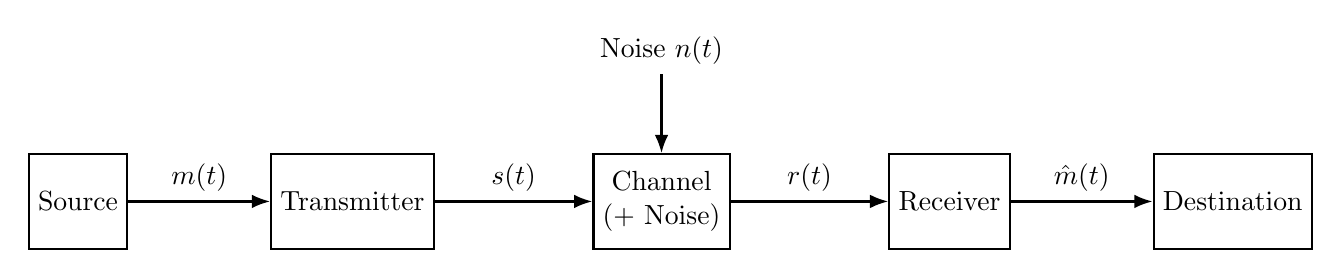
\begin{tikzpicture}[
  block/.style={draw, thick, minimum width=1.0cm, minimum height=1.2cm, align=center},
  >={Latex}
]

% Nodes
\node[block] (src) {Source};
\node[block, right=1.8cm of src] (tx) {Transmitter};
\node[block, right=2.0cm of tx] (ch) {Channel\\(+ Noise)};
\node[block, right=2.0cm of ch] (rx) {Receiver};
\node[block, right=1.8cm of rx] (dst) {Destination};

% Connections
\draw[->, thick] (src) -- (tx) node[midway, above] {$m(t)$};
\draw[->, thick] (tx) -- (ch) node[midway, above] {$s(t)$};
\draw[->, thick] (ch) -- (rx) node[midway, above] {$r(t)$};
\draw[->, thick] (rx) -- (dst) node[midway, above] {$\hat{m}(t)$};

% Noise arrow into channel
\node[above=1.0cm of ch] (n) {Noise $n(t)$};
\draw[->, thick] (n) -- (ch);

\end{tikzpicture}
Above shows a commoly used model for a signle-link communication system. This block diagram is also applicable to remote sensing system, such as radar or sonar, in which the system input and output may be located at the same site.

Befor the Transmitter, we usually have a input transducer.

\textbf{\textit{Input Transmitter}}: Convert the message produced by a source to a form suitable for the particular type of communication system.

\textbf{\textit{Transmiiter}}: The purpose of the transmitter is to couple the message to the channel. In some intercom systems, it is often necessary to \textit{modulate} a carrier wave with the signal from the input trnasducer. \textit{Modulation} is the systematic variation of some attribute of the carrier, such as amplitude, phase, or frequency, in accordance with a function of the message signal. There are several reasons for using a carrier and modulating it.
\begin{itemize}
  \item For ease of radiation.
  \item To reduce noise and interference.
  \item For channel assignment.
  \item For multiplexing or transmission of several messages over a single channel.
  \item To overcome equipment limitations.
\end{itemize}
in addition the modulation. other primart functions performed bt the transmitter are filtering, amplification, and coupling the modulated signal to the channel.

\textbf{\textit{Channel}}: The signal undergoes degradation from transmitter to receiver.

\textbf{\textit{Receiver}}: The receiver's function is to extract the desired message from the receoved signal at the channel output and to convert it to a form suitable for the output transducer.

\textbf{\textit{Output Transducer}}: This output transducer completes the communication system. This devices converts the electric signal at its input into the form desired by the system user.
\section{Channel Characteristics}

\section{Summary of System-Analysis Techniques}

\section{Probablilistic Approaches to System Optimization}
\begin{notebox}[Summary]
some summary
\end{notebox}

\section{Summary}
\begin{notebox}[Thinking]
some thinking
\end{notebox}

\chapter{Chapter 2:}
\section{}
\begin{notebox}[Summary]
some summary
\end{notebox}

\section{}
\begin{notebox}[Concept]
some concept 
\end{notebox}

\section{}
\begin{notebox}[Thinking]
some thinking
\end{notebox}

\end{document}
